\section{Reduced Tuple Search}

In a packet classification problem, rules can be classified into multiple groups and each group is called as a tuple. The lookup process needs to traverse tuples to find the matching rule with the highest priority. Therefore, we need to reduce the number of tuples and the lookup time in each tuple to achieve high lookup speed. In this section, we propose a Mask Length Reduction (MLR) method to reduce the number of tuples, and design a DTC data structure with three priority-based enhancements to reduce the lookup time in each tuple.

\subsection{Mask Length Reduction}

The rules can be divided into multiple tuples by different mask lengths of the source and destination IP addresses. As shown in Figure \ref{mask_length_reduction}, the mask lengths of Rule1 and Rule2 are (24,24), the mask length of Rule3 is (16,24), and the mask length of Rule4 is (16,16). Therefore, the rules are divided into three tuples. \rev{The lookup operation requires traversing the tuples to find the rule with the highest priority.} Each tuple contains a hash table that uses two fields to match the rules, and then applies the chained search to check the \rev{five} fields. \note{Why directly to the remaining three fields? You could also actually search the match of the actual source and destination of rules, right?} For example, the Packet2 \rev{requires traversing three tuples with} three \note{why 3 not 2?} hash searches and a rule check to match Rule4 \rev{in Tuple3}.

To reduce the number of tuples for higher lookup speed, the Mask Length Reduction (MLR) takes two strategies:  reducing the mask length of the rule to a specific value, and merging rules with similar mask lengths into one tuple. In Figure \ref{mask_length_reduction}, MLR reduces the rules with the mask lengths in (16$\sim$24, 16$\sim$24) to (16,16). So Rule1-Rule4 become Rule1'-Rule4', with the mask lengths trimmed to (16,16), and all four rules are placed in a tuple. The Packet2 only performs a hash search and a rule check to match Rule4 in Tuple1'.

Different from TSS and TupleMerge, a tuple in DTC contains the rules with a range of mask lengths and a rule is inserted into only one tuple. In contrast, containing only rules with the same mask length, TSS generates a large number of tuples. As a rule in TupleMerge can be inserted into multiple tuples, it is difficult to manage the tuples, which increases the update speed.


Reducing the number of tuples on the one hand increases the lookup speed, but on the other hand also leads more rules to fall into the same tuple and increases the lookup speed inside the tuple.\note{How to find a tuple? If it is through hashing, not search, will higher number of tuples leads to more searching time? What is slot? You haven't introduced slot yet, right? You kept saying slot here.}\note{(ZCY) I add the tuple traversing in the first paragraph}
%the chain length in the slot and affect the lookup speed. 
For example, Rule1-Rule3 are changed to Rule1'-Rule3' and have the same source IP and destination IP. Therefore, they are indexed to be stored in the same tuple in the hash table and form a chain.

\rev{If a tuple containing too much rules, the lengths of the rule chain will be long, which will affects the lookup speed. Therefore, it is important to consider of both the number of tuples and the lengths of the rule chains. }\note{Do you need to look for step size in this work? You are forming tuples, but didn't do it through the finding of "step size", from what you presented. So this paragraph does not mactch your scheme, although you are looking for the best tuple formulation.}

\begin{figure}[htbp]
\centering
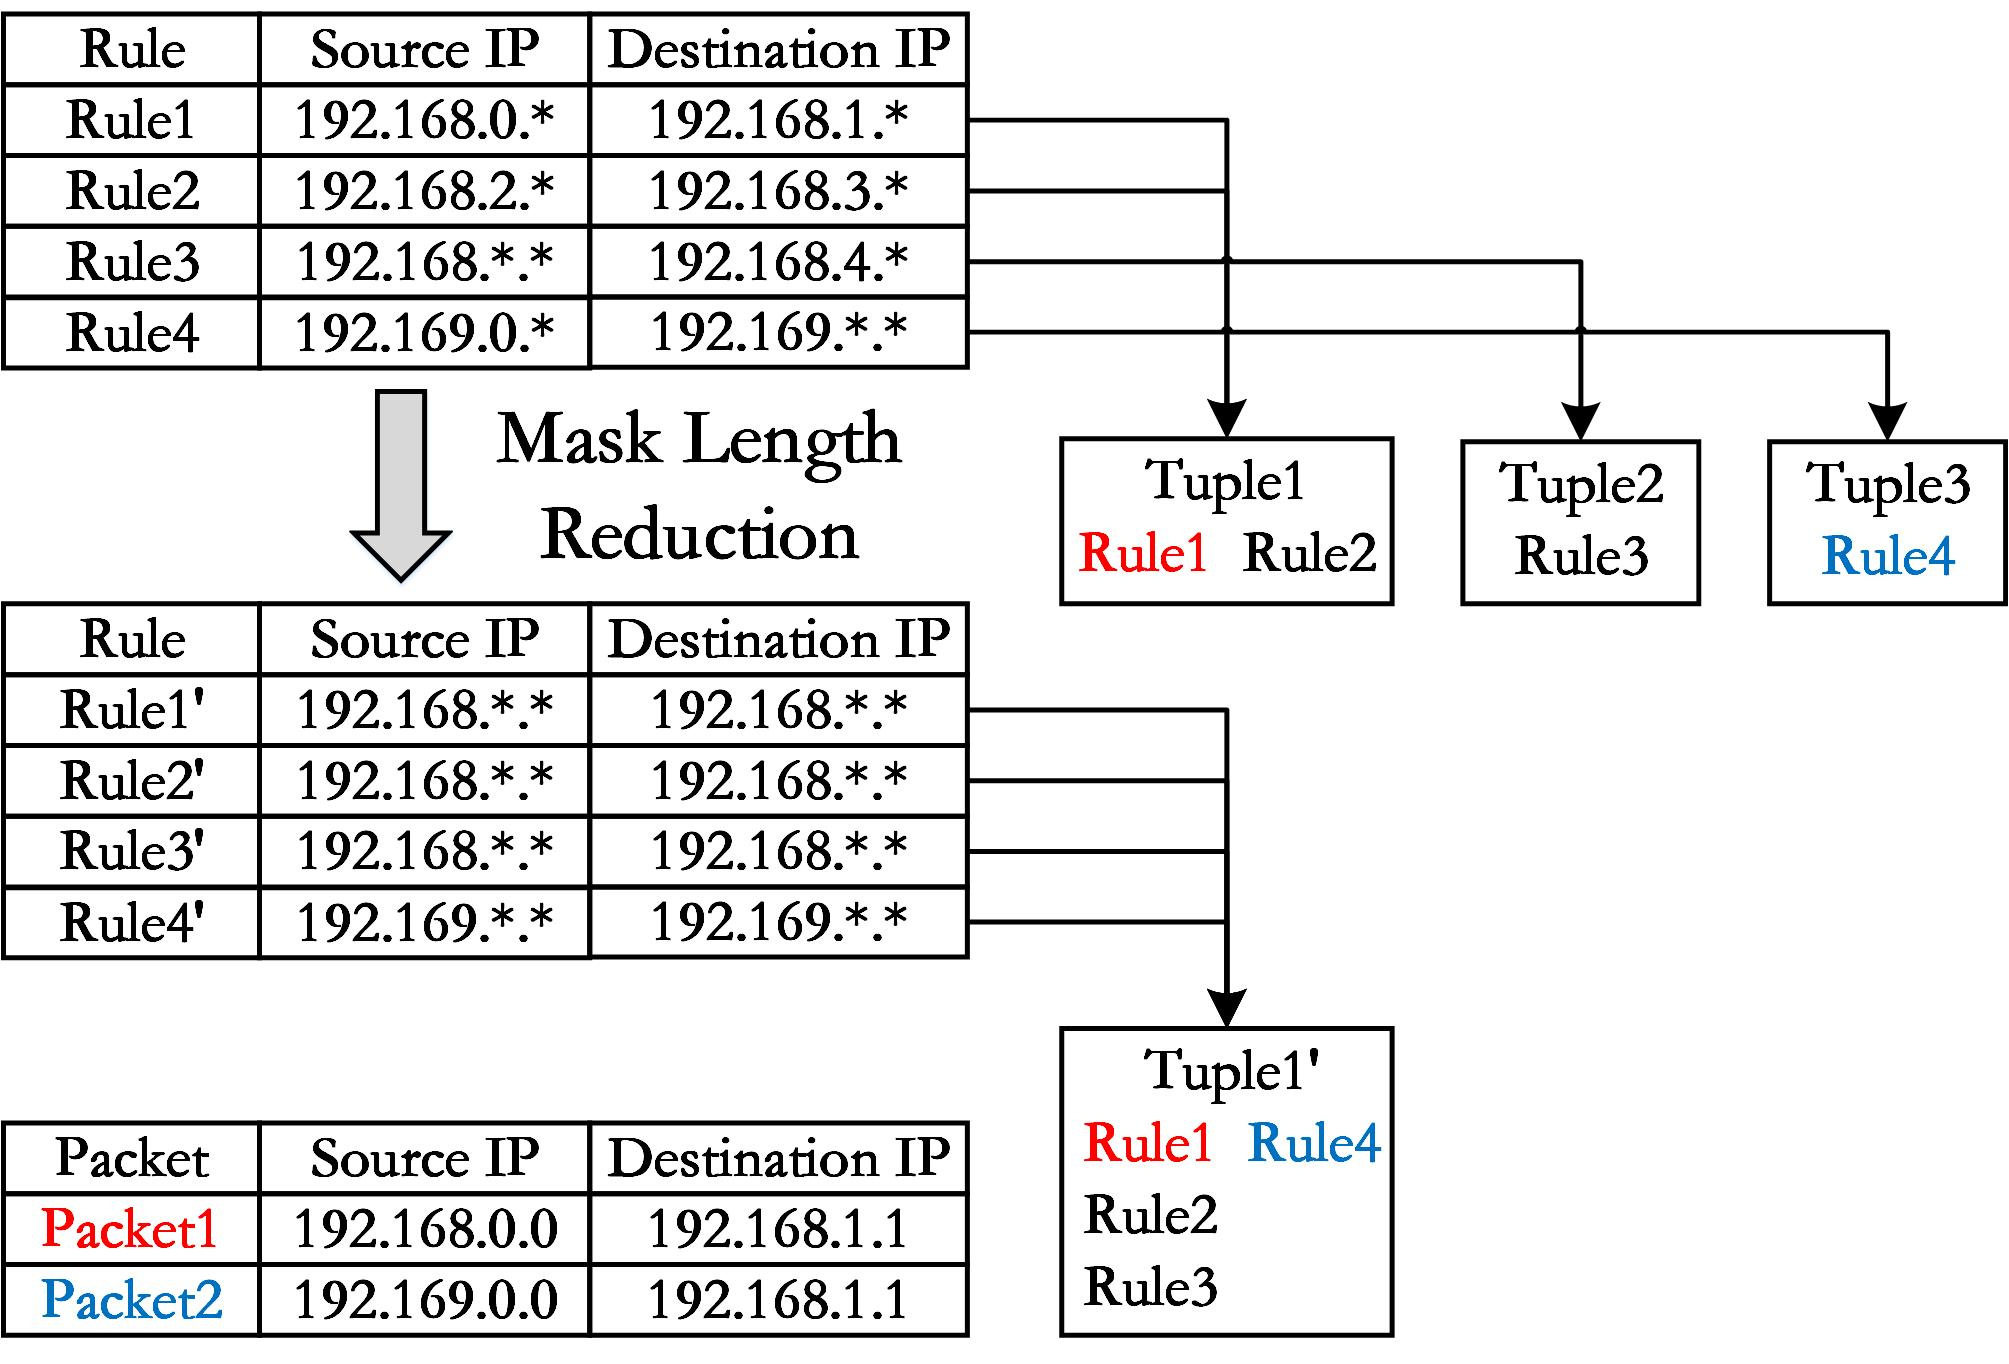
\includegraphics[width=0.9\linewidth]{figure/mask_length_reduction}
\caption{Mask Length Reduction.}
\label{mask_length_reduction}
\end{figure}

\begin{figure}[htbp]
\centering
\includegraphics[width=0.9\linewidth]{figure/basic_DTC}
\caption{Basic DTC data structure.}
\label{basic_DTC}
\end{figure}

\subsection{basic data structure of DTC}

%(TODO: Split the data structure to introduce the slot)

\rev{The basic data structure of DTC consists of four parts: tuples, buckets, slots and rules, as shown in Figure \ref{basic_DTC}. }

\rev{

\textbf{Tuples:} Each tuple contains a hash table which consists of multiple buckets. A tuple only stores the rules with the same mask length of source IP and destination IP address after MLR.

\textbf{Slots:} Each slot applies a chain structure to sotre the rules with the same source and destination IP  after MLR.

\textbf{Buckets:} Each bucket applies a chain structure to store slots. A slot uses its source and destination IP to form a $key$. Then, a $key$ is hashed to be a $hash\_key$, which is 32-bits. Suppose the number of buckets in a tuple is $n$, and the index of the bucket that stores this slot is $hash\_key\%n$. Different slot has different key, however, they can be indexed to the same bucket. 

}

All tuples, rules and slots in DTC data structure are sorted by their priorities. As shown in Figure \ref{basic_DTC}, suppose the rule set contains seven rules Rule1-Rule7 and the priority of Rule$i$ is $i$($e.g.,$Rule7 has the highest priority 7). The priority of each tuple is determined by the highest priority rule in this tuple, and all tuples are sorted according to their priorities from high to low. The priority of each slot is determined by the highest priority rule in this slot, and the slots in each bucket are also sorted according to their priorities from high to low. Each rule has a priority itself, and the rules in each slot are sorted according to their priorities from high to low.

\subsection{DTC lookup and update}
The complete lookup process for a packet in the DTC data structure consists of three steps. First, the packet searches in all tuples. Second, in each tuple, we use the hash function to quickly find the matching slot with the matching source IP and destination IP after MLR. Third, in each matching slot, we check all the rules to find the matching rule with the highest priority. The last matching rule of this packet is the rule with the highest priority among the matching rules in all tuples.

Due to the DTC priority data structure, the lookup process contains three priority optimization methods. The first is the tuple priority optimization. If the priority of the current matching rule is higher than or equal to the current tuple, we can skip the remaining tuples and return this matching rule. The second is the slot priority optimization. If the priority of the current matching rule is higher than or equal to the current slot, we can skip the remaining slots and then continue the lookup process in the next tuple. The third is the rule priority optimization. If the priority of the current matching rule is higher than or equal to the current rule, we can skip the remaining rules and slots, and then continue the lookup process in the next tuple. For example, suppose Packet5 can match both Rule5 and Rule2. In Tuple1, when Packet5 matches Rule5, the priority of the current matching rule is 5, then we skip Rule4 and continue the lookup process in the next tuple by the rule priority optimization. In Tuple2, we check Slot6 and skip Slot2 by the slot priority optimization. In Tuple3, the priority of the matching rule is higher than Tuple3, so we stop the lookup process and return Rule5 by the tuple priority optimization.

The pseudo code for the lookup process is shown in Algorithm \ref{lookup}. $(1)$Line1-2 initialize the matching rule $r$ to $NULL$ and the priority of the matching $pri$ to $-1$. $(2)$Line3-34 are the first step that traverses all tuples. Line5-7 are the tuple priority optimization. Line8-9 calculate the source IP $sip$ and the destination IP $dip$ after MLR. Line10-12 use the hash function of $sip$ and $dip$ to find the indexed bucket in the hash table. $(3)$Line13-33 are the second step that traverses the slot chain to find the matching slot. Line14-16 are the slot priority optimization. $(4)$Line19-29 are the third step that traverses the rule chain to find the matching rule. Line26-28 are the rule priority optimization. $(5)$Finally, the lookup process returns the matching rule $r$ in line35.






\begin{algorithm}
    \caption{The lookup process}
    \label{lookup}
    \KwIn{the array of tuples $tuples$, the number of tuples $tuples\_num$, the packet $packet$\;}
    \KwOut{the matching rule $r$\;}

    $r = NULL$\;
    $pri = -1$\;
    \For{$i = 0;i < tuples\_num; i++$} {
        $tuple = tuples[i]$\;
        \If{$pri \ge tuple.pri$} {
            $break$\;
        }
        $sip = packet.sip \& tuple.sip\_mask$\;
        $dip = packet.dip \& tuple.dip\_mask$\;
        $hash = HashFunction(sip, dip)$\;
        $hashtable = tuple.hashtable$\;
        $slot = hashtable.buckets[hash\&hashtable.mask]$\;
        \While{$slot \neq NULL$} {
            \If{$pri \ge slot.pri$} {
                $break$\;
            }
            \If {$sip == slot.sip$ \textbf{and} $dip == slot.dip$} {
                $rule = slot.rule$\;
                
                \While{$True$} {
                \If {$Match(rule, packet) == True$} {
                        $pri = rule.pri$\;
                        $r = rule$\;
                        $break$\;
                    }
                    $rule = rule.next$\;
                    \If {$rule == NULL$ \textbf{or} $pri \ge rule.pri$} {
                        $break$\;
                    }
                }
                $break$\;
            }
            $slot = slot.next$\;
        }
    }
    return $r$\;
\end{algorithm}

The operation of inserting or deleting a rule is very simple. First, we use the mask lengths of the source IP and the destination IP of this rule to find the corresponding tuple. Then, we perform the insert or delete operation in the hash table of this tuple. If the insert or delete operation changes the priority of the slot or tuple, we adjust the order of the slots or tuples to ensure the DTC priority structure. 